\input{../YKY-preamble.tex}

\usepackage[CJKspace]{xeCJK}
\setCJKmainfont[BoldFont=SimHei,ItalicFont=KaiTi]{SimSun}
\usepackage{color}
\usepackage{hyperref}

\usepackage{mathtools}
\usepackage{hyperref}

\title{GILR -- genetic induction of logic rules \\ {\normalsize white paper}}
% \author{general.intelligence@gmail.com}

\begin{document}
\maketitle

系统分为两部分:
\begin{itemize}
	\item 逻辑规则引擎 (logic rules engine)
	\item 基因算法 逻辑规则学习器 (genetic inductive learning of logic rules)
\end{itemize}

初步 测试 是「打井游戏」(tic-tac-toe),例如:
\begin{equation}
\begin{tabular}{c|c|c}
	$\bigcirc$ &          & $\times$ \\
\hline
	$\bigcirc$ & $\times$ & $\bigcirc$ \\
\hline
	$\times$   & $\times$ & $\bigcirc$ 
\end{tabular}
\end{equation}

\section{Genetic learning of rules}

\subsection{What is a logic rule?}

例如,数学式子可以表示成 tree, $V + F = E + 2$:
\begin{equation}
\vcenter{\hbox{\includegraphics[scale=0.6]{Euler-formula.png}}}
\end{equation}

逻辑 rule 必然包含 $\Rightarrow$,可以将 rule 分成 \textbf{head} 和 \textbf{tail} 两部分:
\begin{equation}
\vcenter{\hbox{\includegraphics[scale=0.6]{I-love-you-n-you-love-me.png}}}
\end{equation}
\begin{equation}
\forall X, Y.  \quad \underbrace{X \heartsuit Y \wedge Y \heartsuit X}_{\mbox{head}} \Rightarrow \underbrace{\smiley X}_{\mbox{tail}}
\end{equation}

\subsection{Genetic algorithm}

要应用 GA 很容易,只需适当地 定义 cross-over 和 mutation.

\textbf{Cross-over}: 随机地选取一个节点,将两个式子在这点交叉。 

\textbf{Mutation}: 随机选择一个节点,在这个节点下换上一棵「随机树」(random tree)

\section{Logic rule engine}

其实这部分和 genetic algorithm 或 learning 都无关,但 logic rules 必需靠 逻辑引擎 运行 才能发生作用。 

逻辑 AI 引擎 的基本运作 如下:
\begin{equation}
\vcenter{\hbox{\includegraphics[scale=0.7]{LBAI-architecture.png}}}
\end{equation}

\subsection{Rete algorithm}

其实这个算法也和学习无关,它只是 逻辑引擎 的一个 \textbf{加速} 算法,大部分 实际使用的逻辑引擎 都需要 Rete 的加速。



\end{document}